

\section{Somaïr}
Dans cette partie, nous allons tout particulièrement nous intéresser au fonctionnement de Somaïr, la mine à ciel ouvert d'Orano au Niger, car c'est la qu'est déployé l'outil CanOp et qui me faut comprendre le fonctionnement pour donner des suggestions cohérentes. Somaïr est une joint venture entre Orano et le Niger.
\subsection{L'exploration}

Le cycle de vie de la mine commence par trouver un gisement exploitable. Le service Geoscience de la mine en est responsable. Il y a une petite équipe d'experts qui en analysant les données géologiques et géopolitiques vont déterminer où on peut mener un projet d'exploitation. Cela peut être une extension sur un gisement connu on va ensuite enregistre des "claims" auprès du gouvernement local pour avoir le droit d'explorer le sous-sol. Un projet d'exploration peut prendre 2~formes~:
\begin{description}
    \item[L'exploration "grass roots"] Dans ce type d'exploration, nous n’avons aucune information sur la zone et il faut donc établir les cartes géologiques et mener un raisonnement sur quel processus géologique aurait pu concentrer l'uranium a un endroit donné. Nous pouvons ensuite faire des forages\footnote{Comme l'uranium est radiactif, nous pouvons approximer la presence de radioactiviter a la precense d'uranium} pour vérifier nos hypothèses. %\footnote{environ \sfrac{3}{4} des forage ne donne aucun resulatat}
    \item[L'exploration "brown fields"]Comme cela fait de nombreuses années que l'on exploite de l'uranium, certaine zone sont déjà eu des forages ou sont à proximité de zone exploitée. On va donc reprendre les données brutes relatives a la zone et chercher quelle supposition on était fait par le passer et si les personnes précédant on néglige quelque chose.
\end{description}
L'étape d'exploration est compliquée, car plus un gisement est concentré alors plus il aura tendance a être petit et donc plus il est difficile a trouvé.

Une fois le gisement trouvé, on va multiplier les forages pour comprendre la forme et la répartition du gisement. Une fois que l'on a atteint un degré de confiance suffisant, le gisement est dit "ressource" et on peut alors passer à l’étape d'extraction.







\subsection{L'extraction}
\label{ssec_extraction}
À Somaïr, la profondeur du gisement, sa forme, la géographie du site et la teneur, on fait que la méthode d'extraction la plus rentable est une mine à ciel ouvert.

On commence par découvrir le gisement, c'est-à-dire d'enlever les 50 à 70~m de roche au-dessus du gisement. Cette roche serait utilisée pour reboucher la mine quand elle arrivera en fin de vie.

L'extraction de l'uranium se fait par "tir". Un tir est une explosion contrôlée qui va briser la roche en morceau plus petit. On délimiter une zone de 50*50*6~m dans lequel on perce des trous tous les 5~m. On utilise d'abord ces trous pour faire une mesure de radiométrie qui va nous permettre d'établir un plan de trie avant de leurs remplir d'explosifs. Une fois les explosifs detoné, un Aide Prospecteur (AP) va mesurer la teneur en uranium de chaque slab\footnote{Un slab est un morceau de roche de 2.5*2.5*0.5m. C'est l'uniter de base de la mine} pour le classer en fonction de sa teneur en uranium.


\subsection{Classification des slabs}
\label{ssec_classification}
\begin{figure}

    \begin{subfigure}[t]{0.4\textwidth}
        \centering
        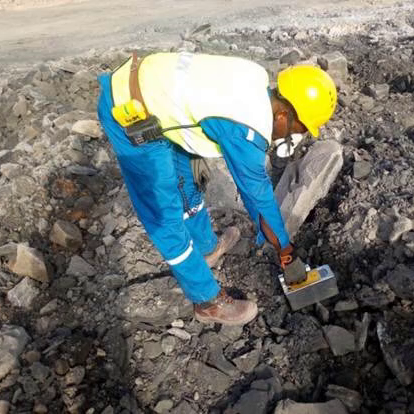
\includegraphics[height=0.3\paperwidth]{photo/Travail_geiger.png}
        \caption{Photo d'un opérateur utilisant un compteur Geiger Müller pour mesurer la teneur en uranium d'un slab}
        \label{fig_AP_geiger}
    \end{subfigure}
    \begin{subfigure}[t]{0.6\textwidth}
        \centering
        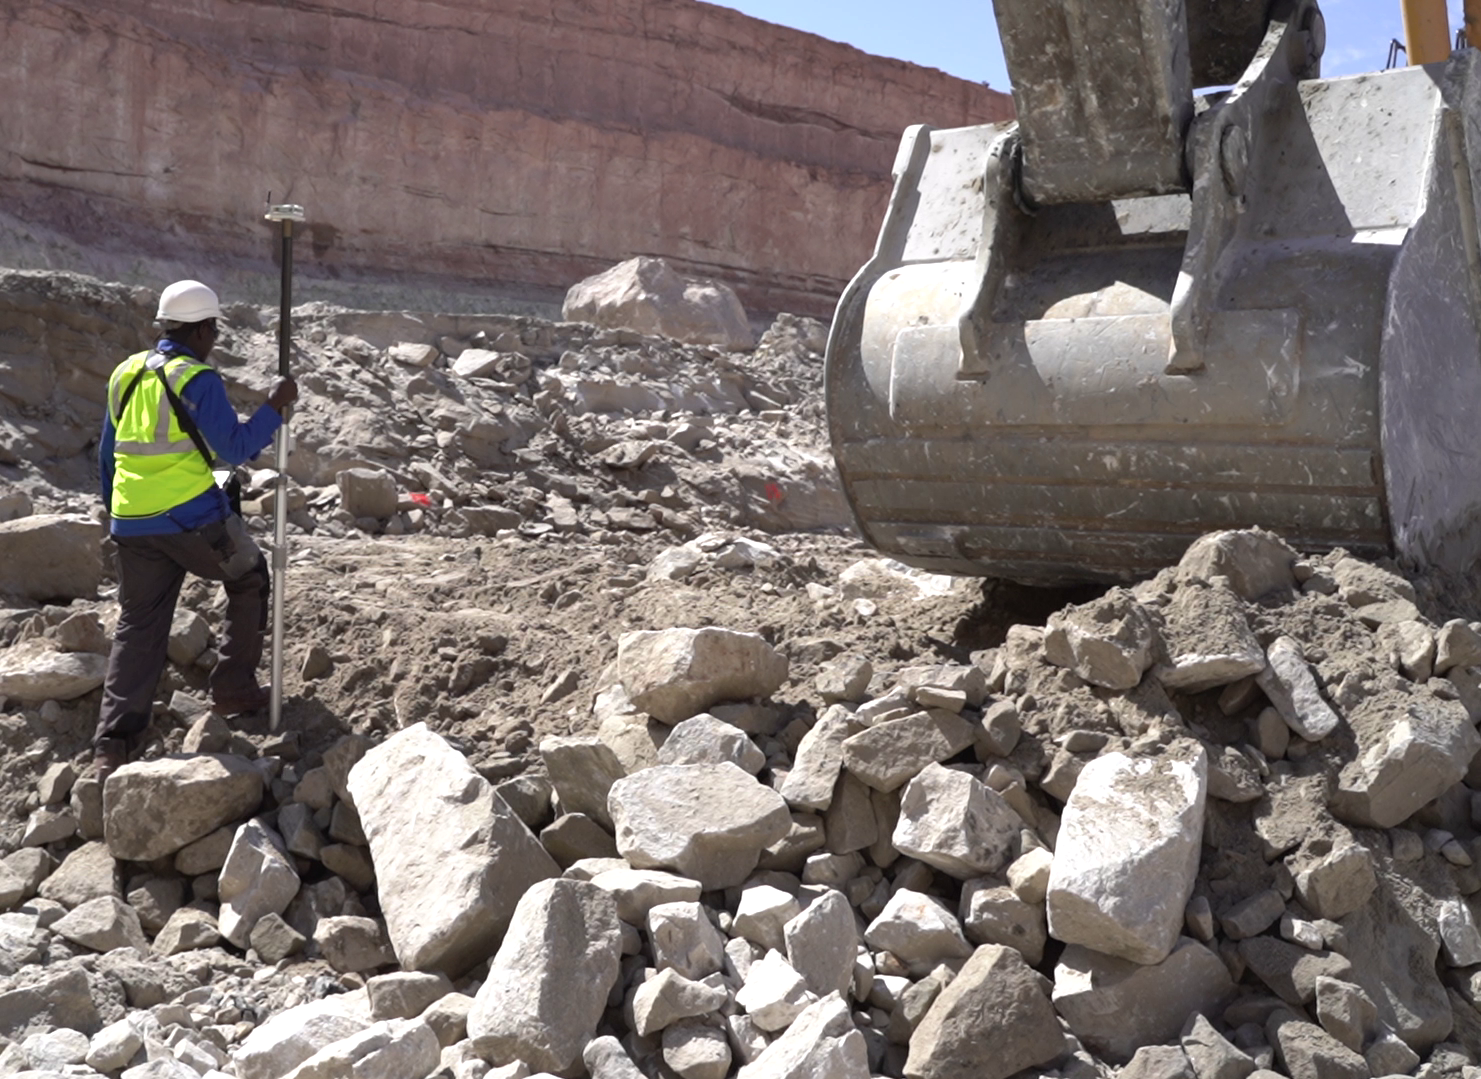
\includegraphics[height=0.3\paperwidth]{photo/CanOp_utilisation.png}
        \caption{Photo d'un opérateur utilisant la CanOp pour mesurer la teneur en uranium d'un slab. Il porte une tablette pour voir les mesures et sa position en temps réel.}
        \label{fig_AP_CanOp}
    \end{subfigure}
    \caption{Photo d'AP utilisant un compteur Geiger Müller et la CanOp}
\end{figure}
Pour savoir comment traiter ces slabs  après extraction, nous les catégorisons en 7~classes de M0 à M6 en fonction de leur teneur en uranium. Les slabs~M0 sont dites stériles, car elle contient tellement peu d'uranium que l'on ne souhaite pas les traiter. Les classes~M1 et M2 subissent un traitement que l'on dit statique, car c'est slab sont empiler et l’on attend que l'uranium descend par gravité jusqu'un bas. Enfin, les slabs de classe supérieure reçoivent un traitement dynamique où en fonction de leur classe elles seront dissoutes avec plus ou moins d'acide selon leurs classes. Il est donc important de bien classer les slabs, car sinon, soit on gaspille  de l'acide ou alors il reste des l'uranium non extrait dans notre refus.
%TODO:mistakes
Avant, pour classer une slab, un Aide Prospecteur (AP) utiliser un compteur Geiger Müller en se penchant pour obtenir des mesures a plusieurs points sur le slab. Il était donc pénible de se pencher en permanence et donc en 2018 a été lancer le projet CanOp pour réduire la pénibilité de la tache et optimiser le tri du minerai.
